\documentclass{article}

% if you need to pass options to natbib, use, e.g.:
\PassOptionsToPackage{numbers, compress}{natbib}
% before loading nips_2016
%
% to avoid loading the natbib package, add option nonatbib:
% \usepackage[nonatbib]{nips_2016}

%\usepackage{nips_2016}
\usepackage[final]{nips_2016}
% to compile a camera-ready version, add the [final] option, e.g.:
% \usepackage[final]{nips_2016}


% The following packages can be found on http:\\www.ctan.org
\usepackage{graphics} % for pdf, bitmapped graphics files
\usepackage{epsfig} % for postscript graphics files
%\usepackage{mathptmx} % assumes new font selection scheme installed
%\usepackage{times} % assumes new font selection scheme installed
\usepackage{amsmath} % assumes amsmath package installed
\usepackage{amssymb}  % assumes amsmath package installed
\usepackage{graphicx}
\usepackage{caption}
\usepackage{float}
\usepackage{subfigure}
\usepackage{color}


\usepackage[utf8]{inputenc} % allow utf-8 input
\usepackage[T1]{fontenc}    % use 8-bit T1 fonts
\usepackage{hyperref}       % hyperlinks
\usepackage{url}            % simple URL typesetting
\usepackage{booktabs}       % professional-quality tables
\usepackage{amsfonts}       % blackboard math symbols
\usepackage{nicefrac}       % compact symbols for 1/2, etc.
\usepackage{microtype}      % microtypography

\renewcommand*{\thesubfigure}{(\arabic{subfigure})}

\title{A graspable object dataset constructed  with the  iCub humanoid robot's camera}

% The \author macro works with any number of authors. There are two
% commands used to separate the names and addresses of multipl
% authors: \And and \AND.
%
% Using \And between authors leaves it to LaTeX to determine where to
% break the lines. Using \AND forces a line break at that point. So,
% if LaTeX puts 3 of 4 authors names on the first line, and the last
% on the second line, try using \AND instead of \And before the third
% author name.



\author{
Murat Kirtay, Ugo Albanese, Egidio Falotico, Cecilia Laschi\\
  The BioRobotics Institute, 
Scuola Superiore Sant'Anna,\\
  56025, Pontedera (PISA), Italy\\
  \texttt{{m.kirtay, u.albanese, e.falotico, c.laschi}@santannapisa.it} \\
  %% examples of more authors
  %%s\And
 %%Ugo Albanese \\
  %% Affiliation \\
  %% Address \\
  %% \texttt{email} \\
  %% \AND
  %% Coauthor \\
  %% Affiliation \\
  %% Address \\
  %% \texttt{email} \\
  %% \And
  %% Coauthor \\
  %% Affiliation \\
  %% Address \\
  %% \texttt{email} \\
  %% \And
  %% Coauthor \\
  %% Affiliation \\
  %% Address \\
  %% \texttt{email} \\
}

\begin{document}
% \nipsfinalcopy is no longer used

\maketitle
%\thispagestyle{empty}
\pagestyle{empty} 


\begin{abstract}
In this technical report, we present the detailed description of a new dataset constructed with the iCub humanoid robot platform and a motorized turntable.  To construct a rotation-invariant dataset, we selected 50 different graspable objects. With the robot camera, we captured images of an object performing a full rotation in steps of approximately 5 degrees. In total, we collected 3600 color images of 50 objects (72 per object). 
\end{abstract}

\section{Introduction}
To construct a new dataset via a robot platform, we followed similar acquisition procedures used for the Columbia Object Image Library (COIL-100)[1].  The dataset contains 72  unprocessed color images for every object (3600 in total).  The objects were selected to be graspable by a robotic hand.  Figure~\ref{fig:rotations} shows one of the objects and some of its poses captured by the iCub robot's camera.  We make the image dataset publicly available to other researchers\footnote{The repository for the dataset and related source code:www.github.com/muratkirtay/icub-camera-dataset}.
Since our ongoing studies rely on this image dataset, the repository will be continuously updated.

\begin{figure}[h!]
\centering
\begin{center}
  \subfigure[ ]{\label{rotations:a}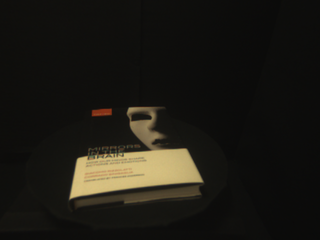
\includegraphics[width=0.15\textwidth]{figs/rotation/1}}
  \subfigure[]{\label{rotations:b}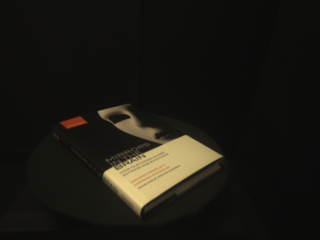
\includegraphics[width=0.15\textwidth]{figs/rotation/10}}
  \subfigure[ ]{\label{rotations:c}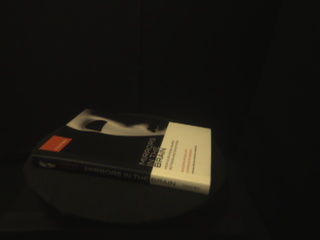
\includegraphics[width=0.15\textwidth]{figs/rotation/20}}
  \subfigure[]{\label{rotations:d}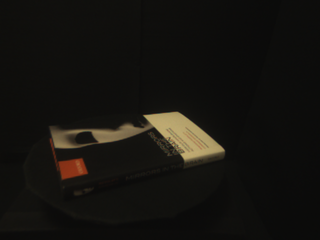
\includegraphics[width=0.15\textwidth]{figs/rotation/30}}\\
  \subfigure[ ]{\label{rotations:e}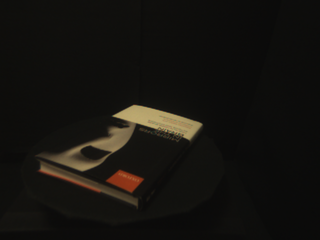
\includegraphics[width=0.15\textwidth]{figs/rotation/40}}
  \subfigure[]{\label{rotations:f}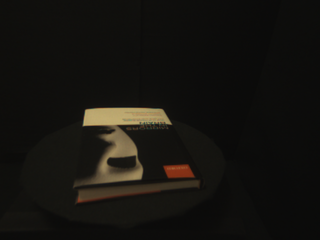
\includegraphics[width=0.15\textwidth]{figs/rotation/50}}
   \subfigure[]{\label{rotations:g}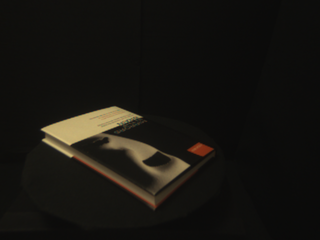
\includegraphics[width=0.15\textwidth]{figs/rotation/60}}
   \subfigure[]{\label{rotations:h}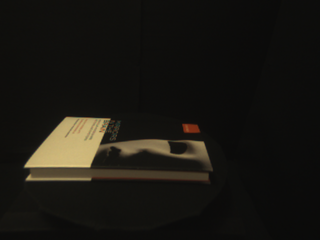
\includegraphics[width=0.15\textwidth]{figs/rotation/70}}
   \end{center}
  \caption{The selected object and in different poses.}
  \label{fig:rotations}
\end{figure}

\begin{figure}
\centering
\begin{center}
  \subfigure[ ]{\label{cmat:a}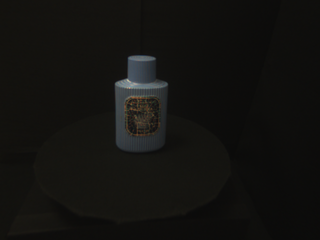
\includegraphics[width=0.15\textwidth]{figs/objects/1}}
  \subfigure[]{\label{cmat:b}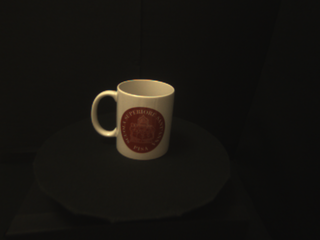
\includegraphics[width=0.15\textwidth]{figs/objects/2}}
  \subfigure[ ]{\label{cmat:c}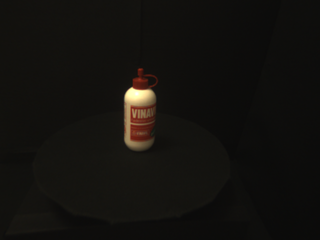
\includegraphics[width=0.15\textwidth]{figs/objects/3}}
  \subfigure[]{\label{cmat:d}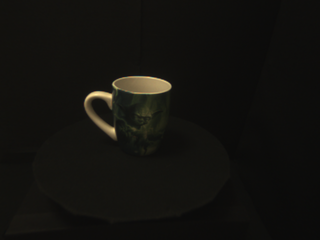
\includegraphics[width=0.15\textwidth]{figs/objects/4}}
  \subfigure[ ]{\label{cmat:e}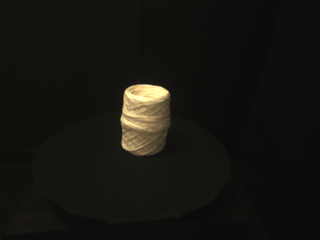
\includegraphics[width=0.15\textwidth]{figs/objects/5}}\\
  \subfigure[]{\label{cmat:f}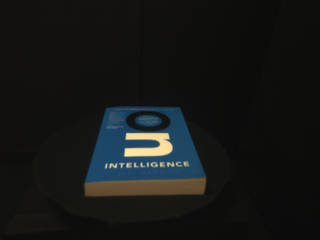
\includegraphics[width=0.15\textwidth]{figs/objects/6}}
   \subfigure[]{\label{cmat:f}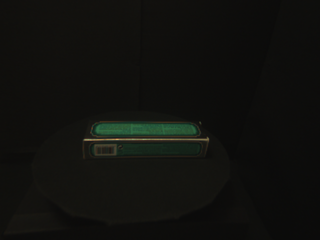
\includegraphics[width=0.15\textwidth]{figs/objects/7}}
   \subfigure[]{\label{cmat:f}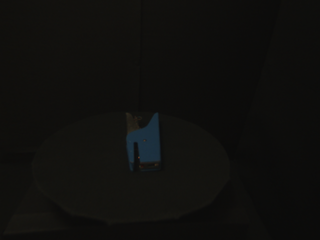
\includegraphics[width=0.15\textwidth]{figs/objects/8}}
   \subfigure[]{\label{cmat:f}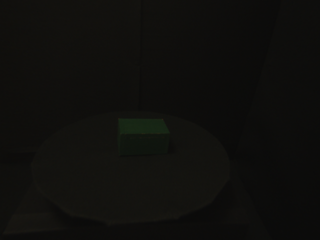
\includegraphics[width=0.15\textwidth]{figs/objects/9}}
   \subfigure[]{\label{cmat:f}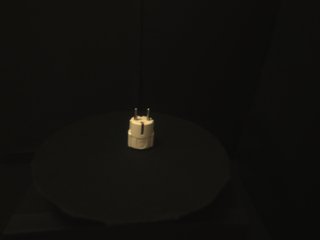
\includegraphics[width=0.15\textwidth]{figs/objects/10}}\\
    \subfigure[]{\label{cmat:f}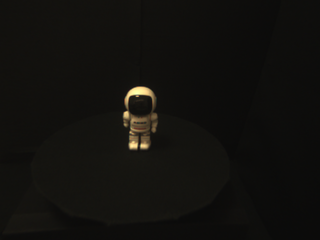
\includegraphics[width=0.15\textwidth]{figs/objects/11}}
    \subfigure[]{\label{cmat:f}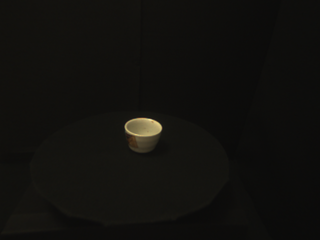
\includegraphics[width=0.15\textwidth]{figs/objects/12}}
    \subfigure[]{\label{cmat:f}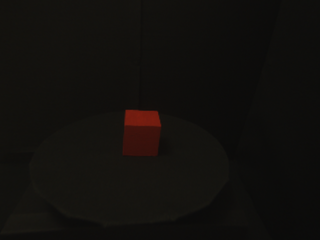
\includegraphics[width=0.15\textwidth]{figs/objects/13}}
   \subfigure[]{\label{cmat:f}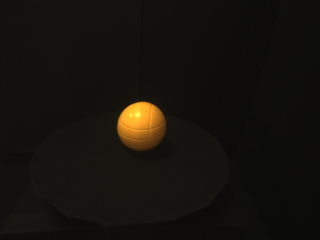
\includegraphics[width=0.15\textwidth]{figs/objects/14}}
    \subfigure[]{\label{cmat:f}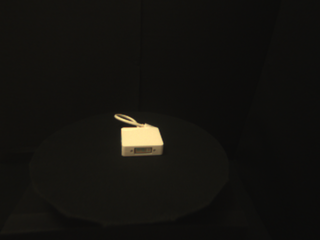
\includegraphics[width=0.15\textwidth]{figs/objects/15}}\\
    \subfigure[]{\label{cmat:f}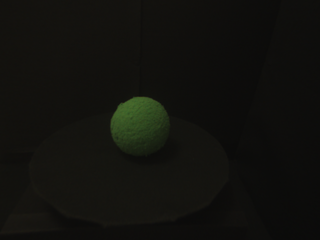
\includegraphics[width=0.15\textwidth]{figs/objects/16}}
    \subfigure[]{\label{cmat:f}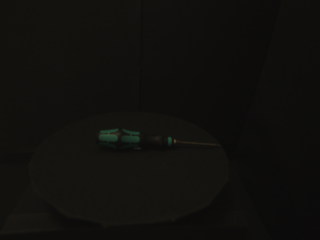
\includegraphics[width=0.15\textwidth]{figs/objects/17}}
    \subfigure[]{\label{cmat:f}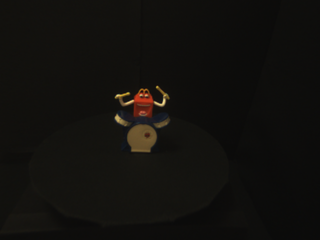
\includegraphics[width=0.15\textwidth]{figs/objects/18}}
    \subfigure[]{\label{cmat:f}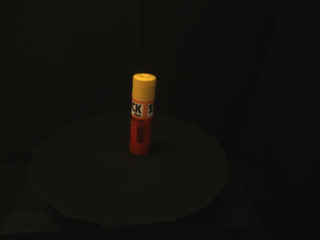
\includegraphics[width=0.15\textwidth]{figs/objects/19}}
    \subfigure[]{\label{cmat:f}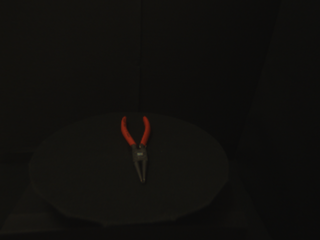
\includegraphics[width=0.15\textwidth]{figs/objects/20}}\\
     \subfigure[]{\label{cmat:f}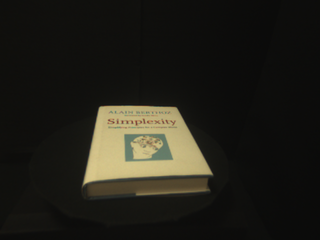
\includegraphics[width=0.15\textwidth]{figs/objects/21}}
     \subfigure[]{\label{cmat:f}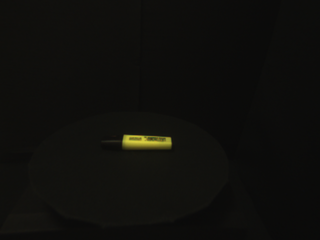
\includegraphics[width=0.15\textwidth]{figs/objects/22}}
     \subfigure[]{\label{cmat:f}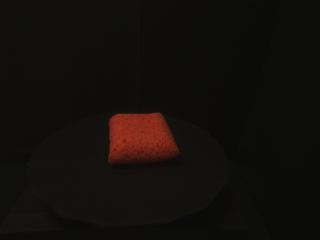
\includegraphics[width=0.15\textwidth]{figs/objects/23}}
    \subfigure[]{\label{cmat:f}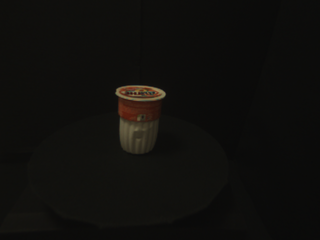
\includegraphics[width=0.15\textwidth]{figs/objects/24}}
    \subfigure[]{\label{cmat:f}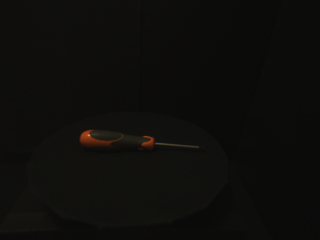
\includegraphics[width=0.15\textwidth]{figs/objects/25}}\\
    \subfigure[]{\label{cmat:f}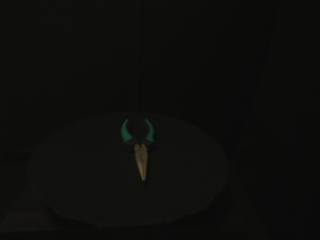
\includegraphics[width=0.15\textwidth]{figs/objects/26}}
     \subfigure[]{\label{cmat:f}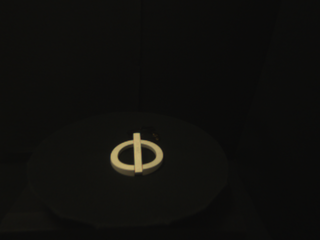
\includegraphics[width=0.15\textwidth]{figs/objects/27}}
     \subfigure[]{\label{cmat:f}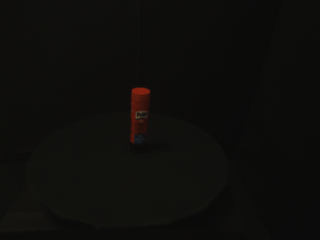
\includegraphics[width=0.15\textwidth]{figs/objects/28}}
    \subfigure[]{\label{cmat:f}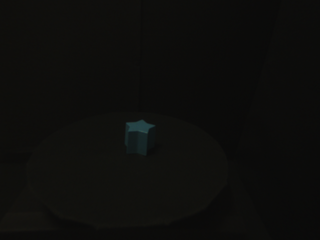
\includegraphics[width=0.15\textwidth]{figs/objects/29}}
    \subfigure[]{\label{cmat:f}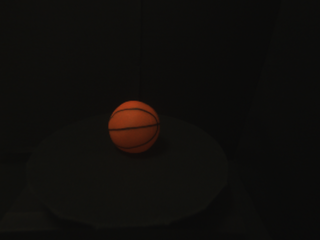
\includegraphics[width=0.15\textwidth]{figs/objects/30}}\\ 
   \subfigure[]{\label{cmat:f}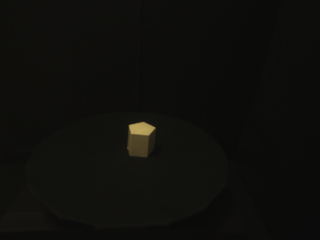
\includegraphics[width=0.15\textwidth]{figs/objects/31}}
   \subfigure[]{\label{cmat:f}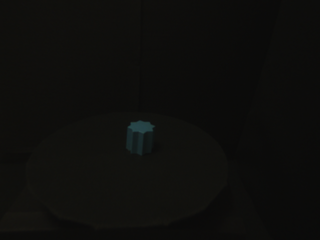
\includegraphics[width=0.15\textwidth]{figs/objects/32}}
   \subfigure[]{\label{cmat:f}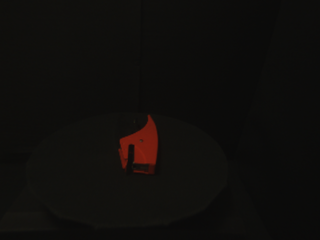
\includegraphics[width=0.15\textwidth]{figs/objects/33}}
    \subfigure[]{\label{cmat:f}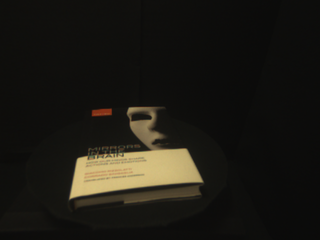
\includegraphics[width=0.15\textwidth]{figs/objects/34}}
     \subfigure[]{\label{cmat:f}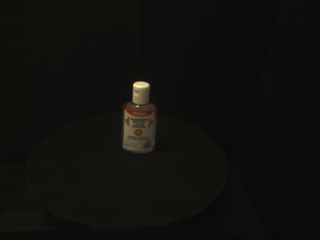
\includegraphics[width=0.15\textwidth]{figs/objects/35}}\\
      \subfigure[]{\label{cmat:f}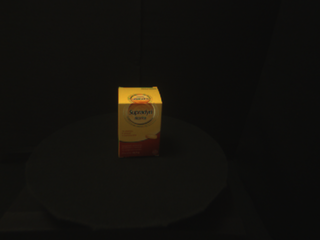
\includegraphics[width=0.15\textwidth]{figs/objects/36}}
       \subfigure[]{\label{cmat:f}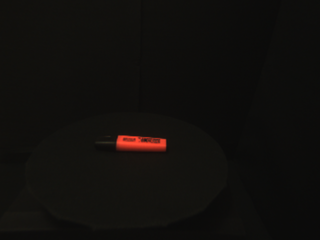
\includegraphics[width=0.15\textwidth]{figs/objects/37}}
        \subfigure[]{\label{cmat:f}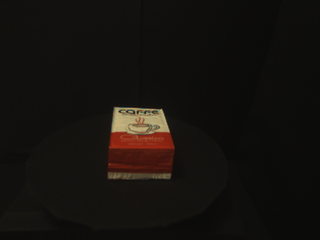
\includegraphics[width=0.15\textwidth]{figs/objects/38}}
        \subfigure[]{\label{cmat:f}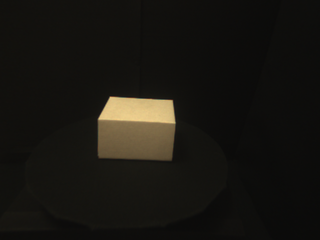
\includegraphics[width=0.15\textwidth]{figs/objects/39}}
        \subfigure[]{\label{cmat:f}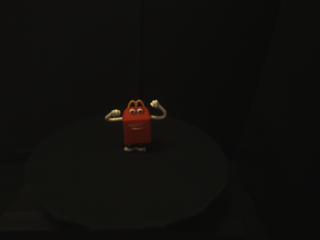
\includegraphics[width=0.15\textwidth]{figs/objects/40}} \\
         \subfigure[]{\label{cmat:f}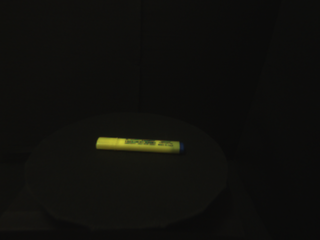
\includegraphics[width=0.15\textwidth]{figs/objects/41}}   
        \subfigure[]{\label{cmat:f}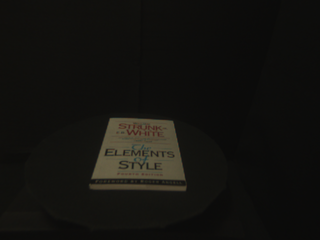
\includegraphics[width=0.15\textwidth]{figs/objects/42}}   
        \subfigure[]{\label{cmat:f}\includegraphics[width=0.15\textwidth]{figs/objects/43}}   
       \subfigure[]{\label{cmat:f}\includegraphics[width=0.15\textwidth]{figs/objects/44}}   
       \subfigure[]{\label{cmat:f}\includegraphics[width=0.15\textwidth]{figs/objects/45}} \\   
        \subfigure[]{\label{cmat:f}\includegraphics[width=0.15\textwidth]{figs/objects/46}}   
         \subfigure[]{\label{cmat:f}\includegraphics[width=0.15\textwidth]{figs/objects/47}}   
          \subfigure[]{\label{cmat:f}\includegraphics[width=0.15\textwidth]{figs/objects/48}}   
           \subfigure[]{\label{cmat:f}\includegraphics[width=0.15\textwidth]{figs/objects/49}}   
            \subfigure[]{\label{cmat:f}\includegraphics[width=0.15\textwidth]{figs/objects/50}}   
   \end{center}
  \caption{Collected images that captured from robot's camera at initial pose}
  \label{fig:objects}
\end{figure}

\section{Hardware setup and image Acquisition}
The acquisition setup consists of the iCub humanoid robot and a motorized turntable. The setup can be seen in Figure~\ref{fig:expsetup}.  The data acquisition procedure begins with placing an object on the turntable; the object is, then, rotated by approximately 5 degrees while capturing an image with the iCub's camera located in the left eye of the robot. 
The Yet Another Robot Platform (YARP) middleware and its Python binding were used to capture raw image data  (RGB pixel matrices). The obtained data were converted to the PNG format.  This procedure was repeated until the turntable completes a full rotation.  The same process is repeated automatically for each object in the dataset. At the end of this acquisition procedure, we captured 3600 color images (with the size of 640x480) and selected samples from the dataset are shown in the Figure~\ref{fig:objects}.
\begin{figure}[h]
	\centering
	\begin{center}
		\label{fig:a}\includegraphics[width=0.4\textwidth]{figs/icub4}
	\end{center}
	\caption{Experiment setup: iCub and motorized turntable}
	\label{fig:expsetup}
\end{figure} 
 
\subsubsection*{Acknowledgments}
We would like to thank Andrea Pratesi, Mariangela Manti, and Taimoor Shah Hassan for their help during various stages of the data acquisition procedure.

\section*{References}

%References follow the acknowledgments. Use unnumbered first-level
%heading for the references. Any choice of citation style is acceptable
%as long as you are consistent. It is permissible to reduce the font
%size to \verb+small+ (9 point) when listing the references. {\bf
%  Remember that you can use a ninth page as long as it contains
%  \emph{only} cited references.}
%\medskip%

\small

[1] S. A. Nene, S. K. Nayar, and H. Murase, ''Object image library (coil- 100,” Tech. Rep., 1996.



\end{document}
